\hypertarget{solveble-representations}{%
\section{Solvable representations}\label{solvable-representations}}

\begin{quote}
Abstractions with structure that is easily solvable.
\end{quote}

While there are other ways to add exploitable structure, here we only
consider linearity.

The bellman equation is a non-linear optimisation problem. It does have
some nice properties, like having a unique optima under the bellman
operator. But, in general, it isn't very friendly. Is there a way to
turn this into a linear problem? What sacrifices need to be made to
achieve this?

\hypertarget{why-linear}{%
\subsection{Why linear?}\label{why-linear}}

\begin{itemize}
\tightlist
\item
  it has many mathematical tools for analysis.
\item
  we know linear systems can be solved efficiently.
\item
  ?
\end{itemize}

Linearity is a nice property that makes optimisation simpler and more
efficient: Linear programming (see appendix: LP)
Solving a system of linear relationships. Has a complexity of ???.
In fact. MDPs can actually be solved via LP. see {[}appendix{]}.

\hypertarget{a-closer-look-at-lmdps}{%
\subsection{A closer look at LMDPs}\label{a-closer-look-at-lmdps}}

(the Todorov ones\ldots{})

The three steps of abstraction - relaxation (transform to a new domain)
- linearisation (and solve) -

\hypertarget{lmdps-more-formally}{%
\paragraph{LMDPs; more formally}\label{lmdps-more-formally}}

\begin{figure}
\centering
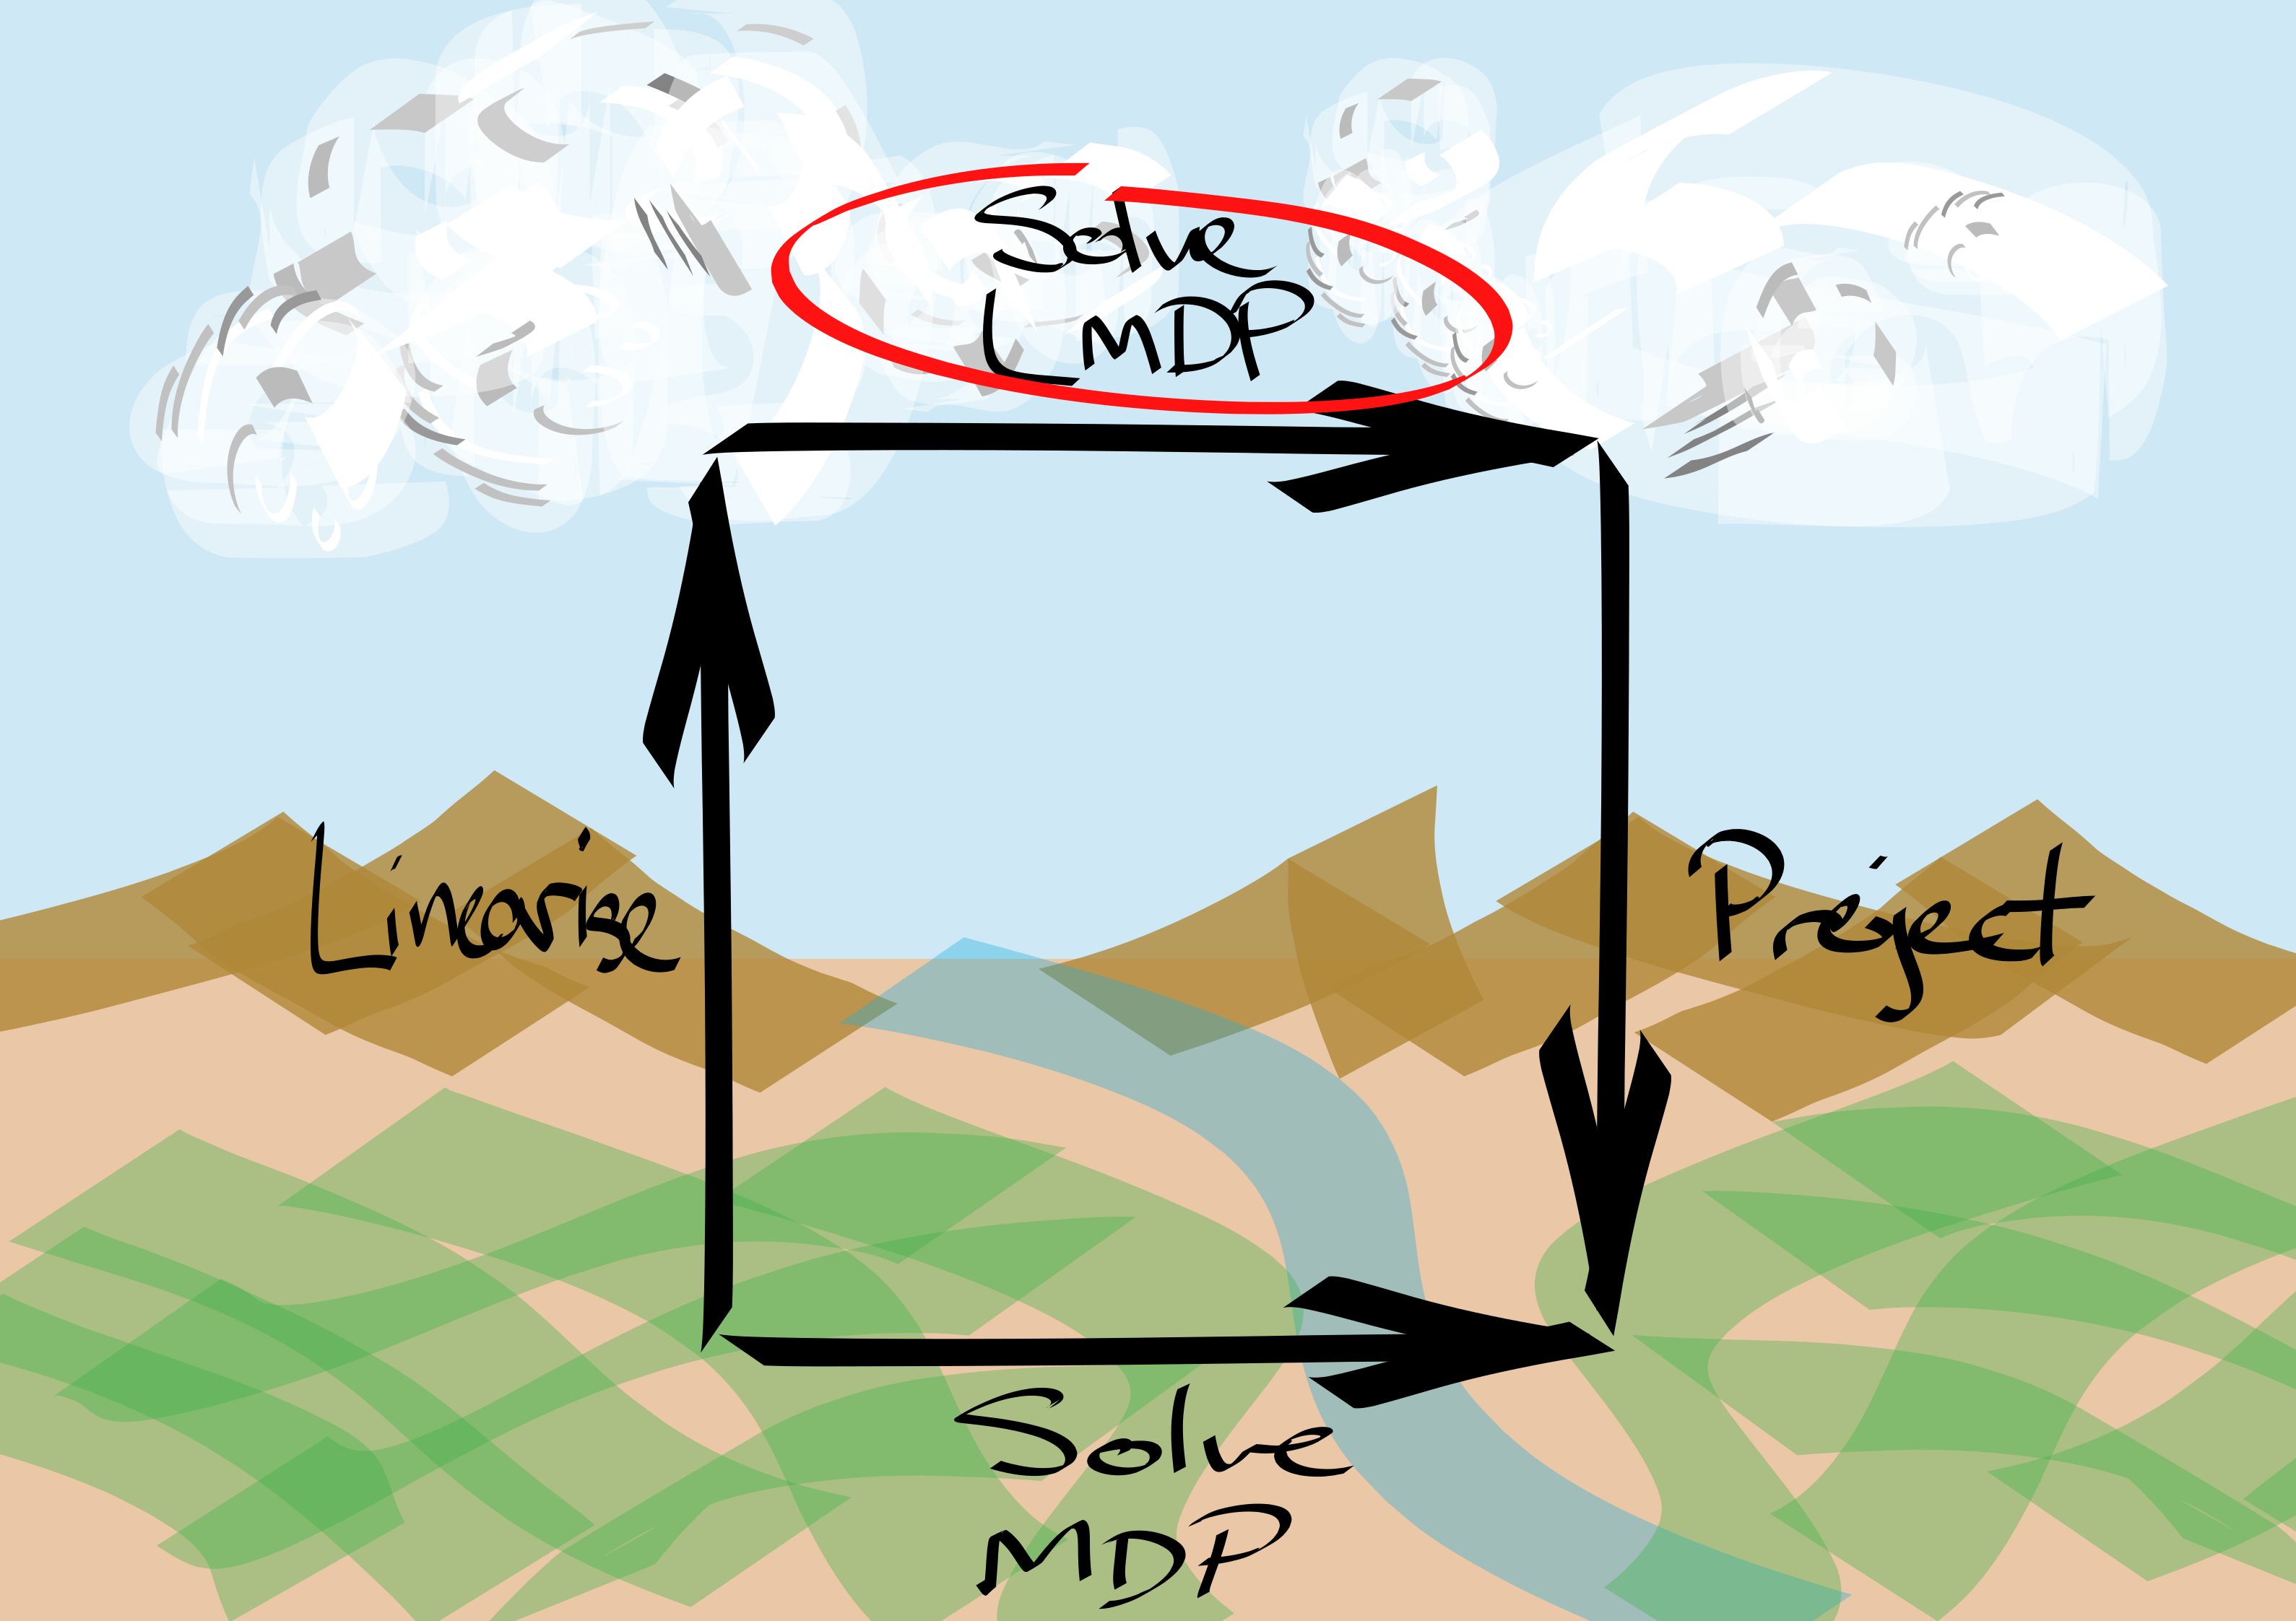
\includegraphics[width=1\textwidth,height=0.5\textheight]{../../pictures/drawings/abstract-representations-solve.png}
\caption{'Solving the LMDP'}
\end{figure}

Rather than picking action from our action space, we are going to pick actions in
 the space of possible transitions from the current state to the next state. Note
 that these transitions are not (yet) constrained to be possible.

We can formulate a linearised markov decision process as;

\begin{align}
V(s) &= \mathop{\text{max}}_{u} q(s) - \text{KL}(u(\cdot| s) \parallel p(\cdot | s)) + \gamma \mathop{\mathbb E}_{s' \sim u(\cdot | s)} V(s') \tag{1}\\
\\
u^{* }(\cdot | s) &= \frac{p(\cdot | s)\cdot z(\cdot)^{\gamma}}{\sum_{s'} p(s' | s) z(s')^{\gamma}} \tag{8}\\
z_{u^{* }} &= e^{q(s)}\cdot P z_{u^{* }}^{\gamma} \tag{11}\\
\end{align}

By definition, an LMDP is the optimisation problem in (1). (3) Define a
new variable, \(z(s) = e^{v(s)}\). (5) Define a new variable that will
be used to normalise \(p(s' | s)z(s')^{\gamma}\). (8) Set the optimal
policy to minimise the KL distance term. (9) Since we picked the optimal
control to be the form in (8), the KL divergence term is zero. (11)
Rewrite the equations for the tabular setting, giving a \(z\) vector,
uncontrolled dynamics matrix.

(see appendix ?? for a full derivation)

\newpage

\hypertarget{a-relaxed-mdp}{%
\subsection{A relaxed MDP}\label{a-relaxed-mdp}}

\begin{figure}
\centering
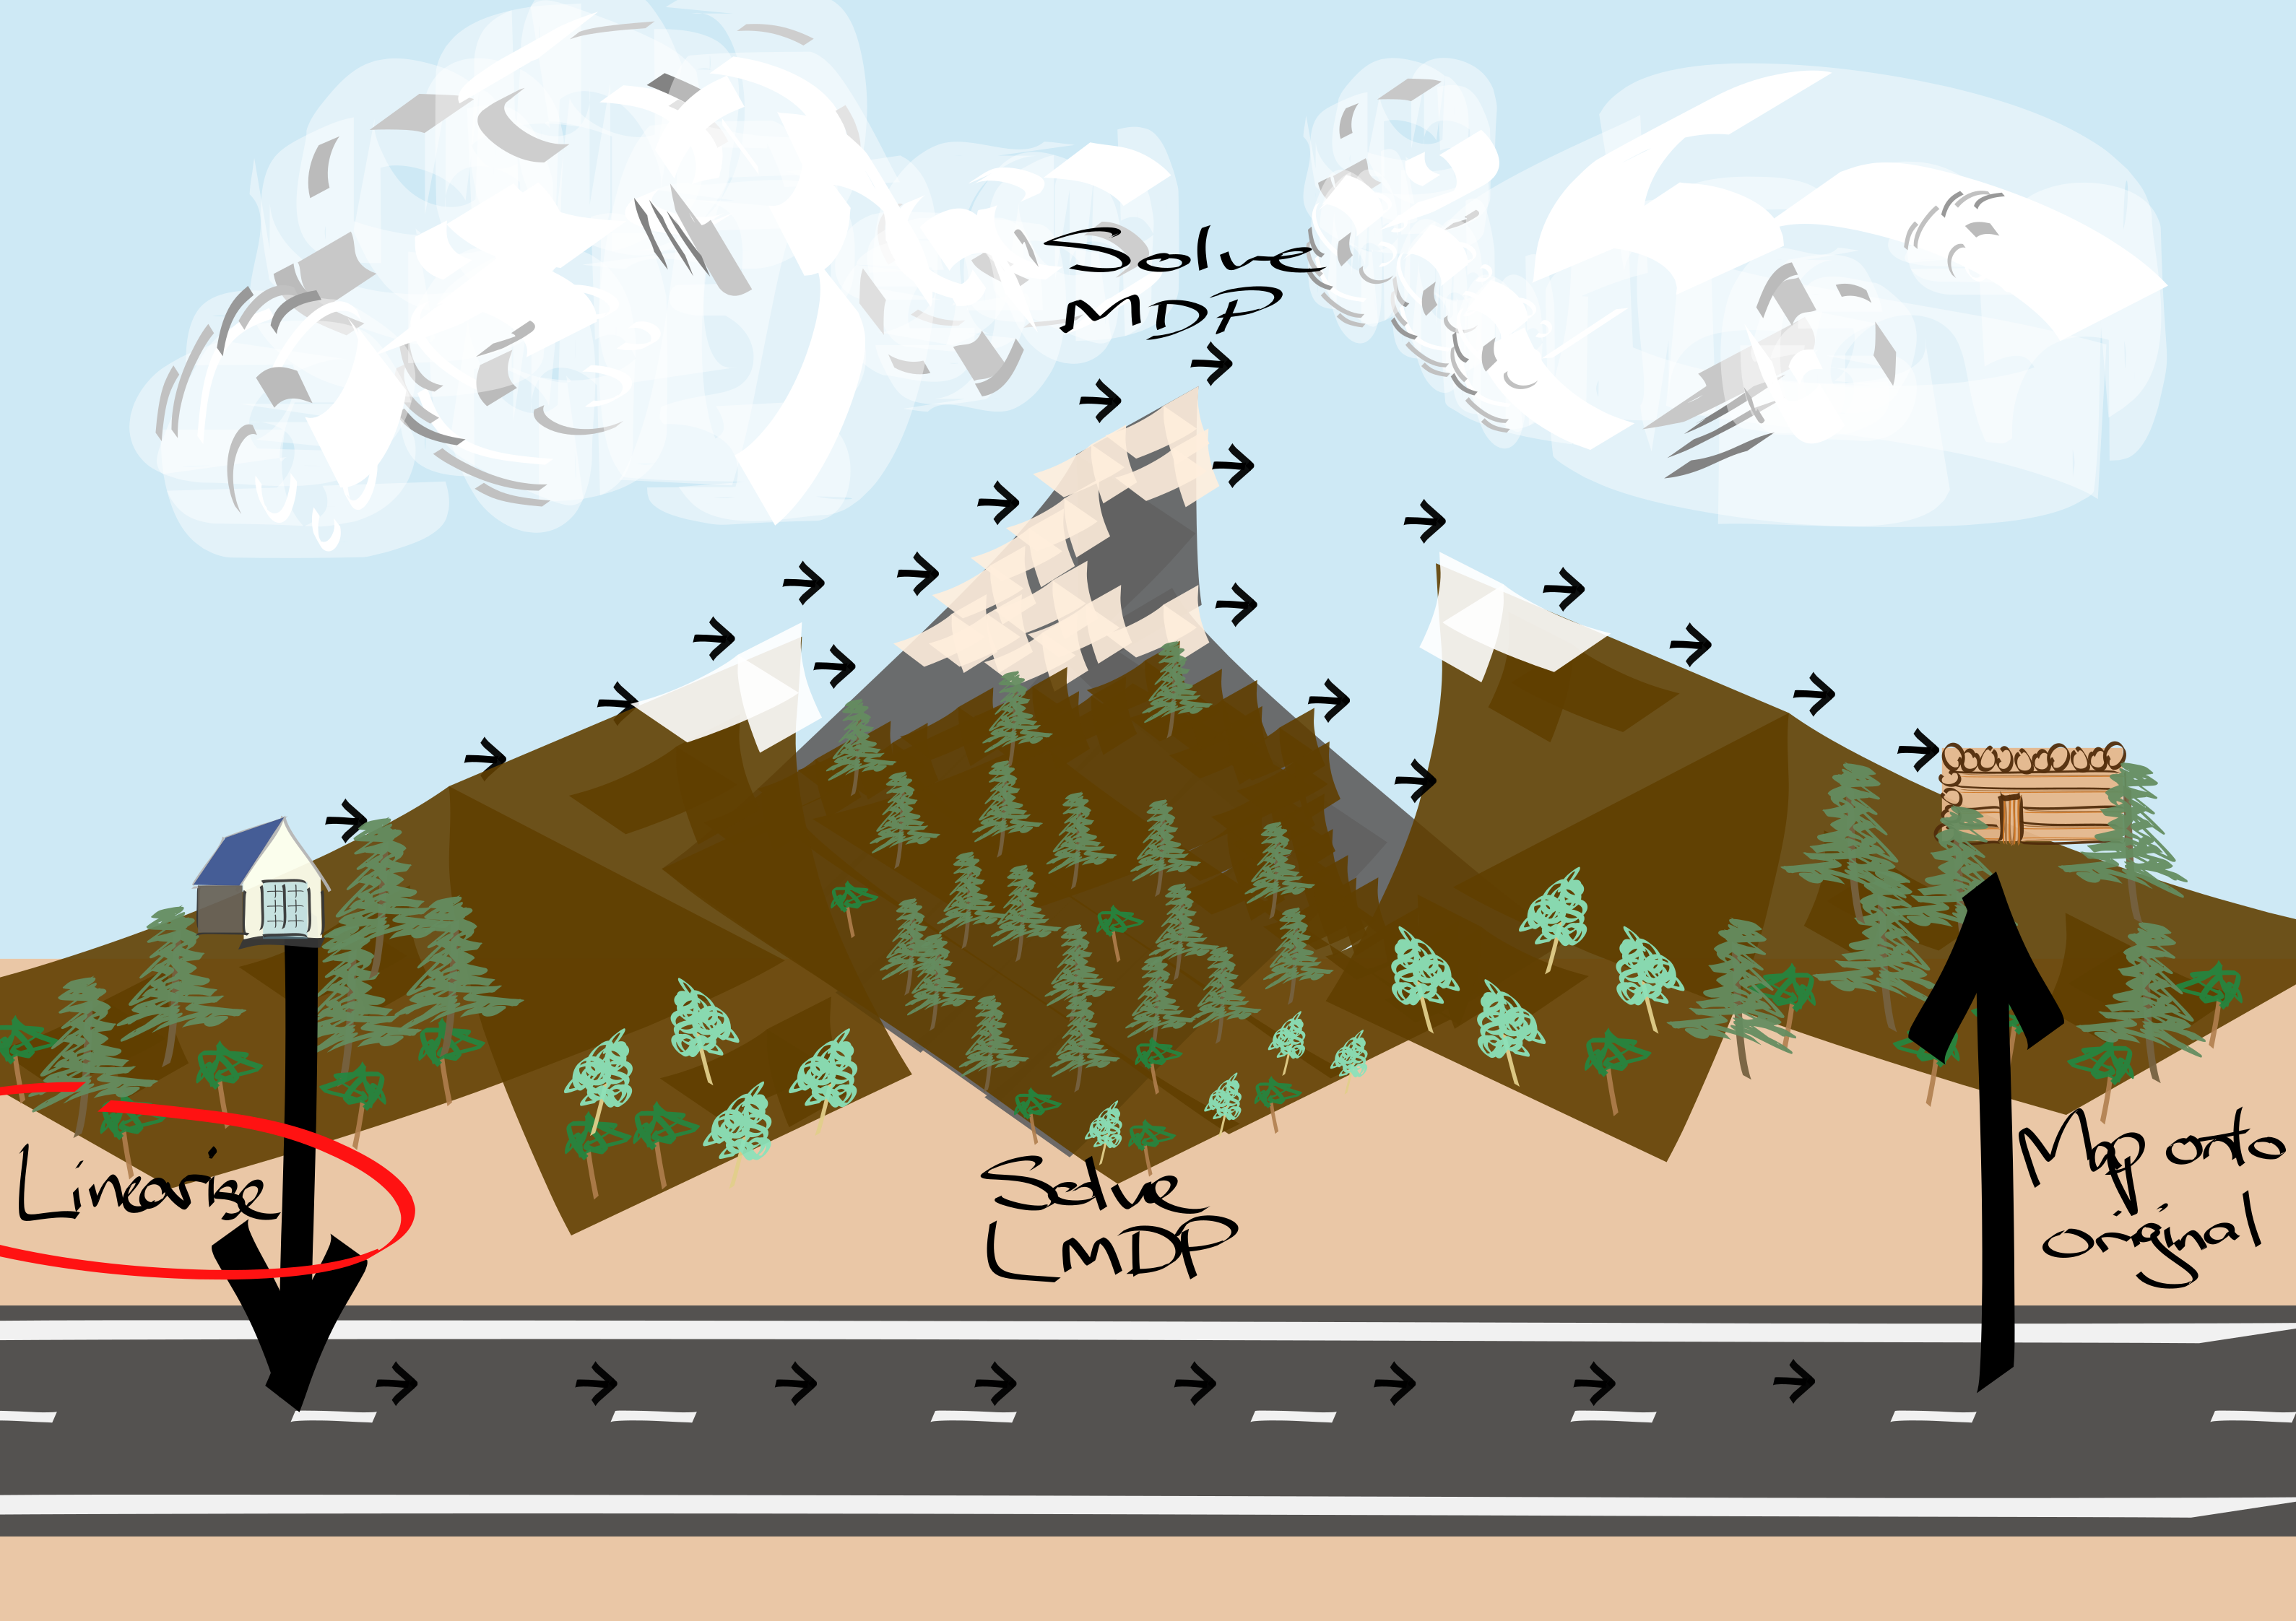
\includegraphics[width=1\textwidth,height=0.5\textheight]{../../pictures/drawings/abstract-representations-linear.png}
\caption{''}
\end{figure}

\begin{quote}
Ok great, we can solve LMDPs. But how does being able to solve an LMDP
help us solve MDPs?
\end{quote}

We want a way to transform a MDP into a LMDP, while preserving the
`structure' of the MDP. But what do we mean by a MDP's structure?

The LMDP, \(\{S, p, q, \gamma\}\) should;

\begin{itemize}
\tightlist
\item
  be able to represent the same transition dynamics as the original MDP,
\item
  give the the same rewards was the original MDP,
\item
  have the same optima.
\end{itemize}

(It turns out that (1) and (2) imply (3) given some assumptions. See
\href{}{Optimality})

So, given a reward function, \(r\), and a transition function, \(P\),
from the MDP, we must translate them into a \(p\) and a \(q\). Thus we
have built a LMDP with the same `structure'.

\begin{align}
\forall s, s' \in S, \forall a \in A, \exists u_a& \;\;\text{such that;} \\
P(s' | s, a) &= u_a(s'|s)p(s'|s) \tag{1}\\
r(s, a) &= q(s) - \text{KL}(P(\cdot | s, a) \parallel u_a(\cdot| s) ) \tag{2}\\
\end{align}

Which leads to \(|A|\) linear equations to solve, for each state in the
MDP.

See appendix {[}{]} for more details.

Alternative views of linearisation.

\begin{itemize}
\tightlist
\item
  A relaxation of the MDP
\item
  Linelihood interpretation
\end{itemize}

\hypertarget{unconstrained-dynamics-and-state-rewards}{%
\subsection{Unconstrained dynamics and state
rewards}\label{unconstrained-dynamics-and-state-rewards}}

\begin{quote}
Let's try and understand this thing we have contructed.
\end{quote}

The state rewards are not capable of giving rewards for actions taken.
Rather, the differences in reward, by taking another action, is captured
by the KL divergence between the control and the unconstrained dynamics.

\begin{itemize}
\tightlist
\item
  What is their function?
\item
  What do they look like?
\end{itemize}

Does it make sense to treat the q(s) like rewards?! They reward for bing
in state s. But cant capture action specific rewards!?

\hypertarget{decoding}{%
\paragraph{Decoding}\label{decoding}}

\begin{figure}
\centering
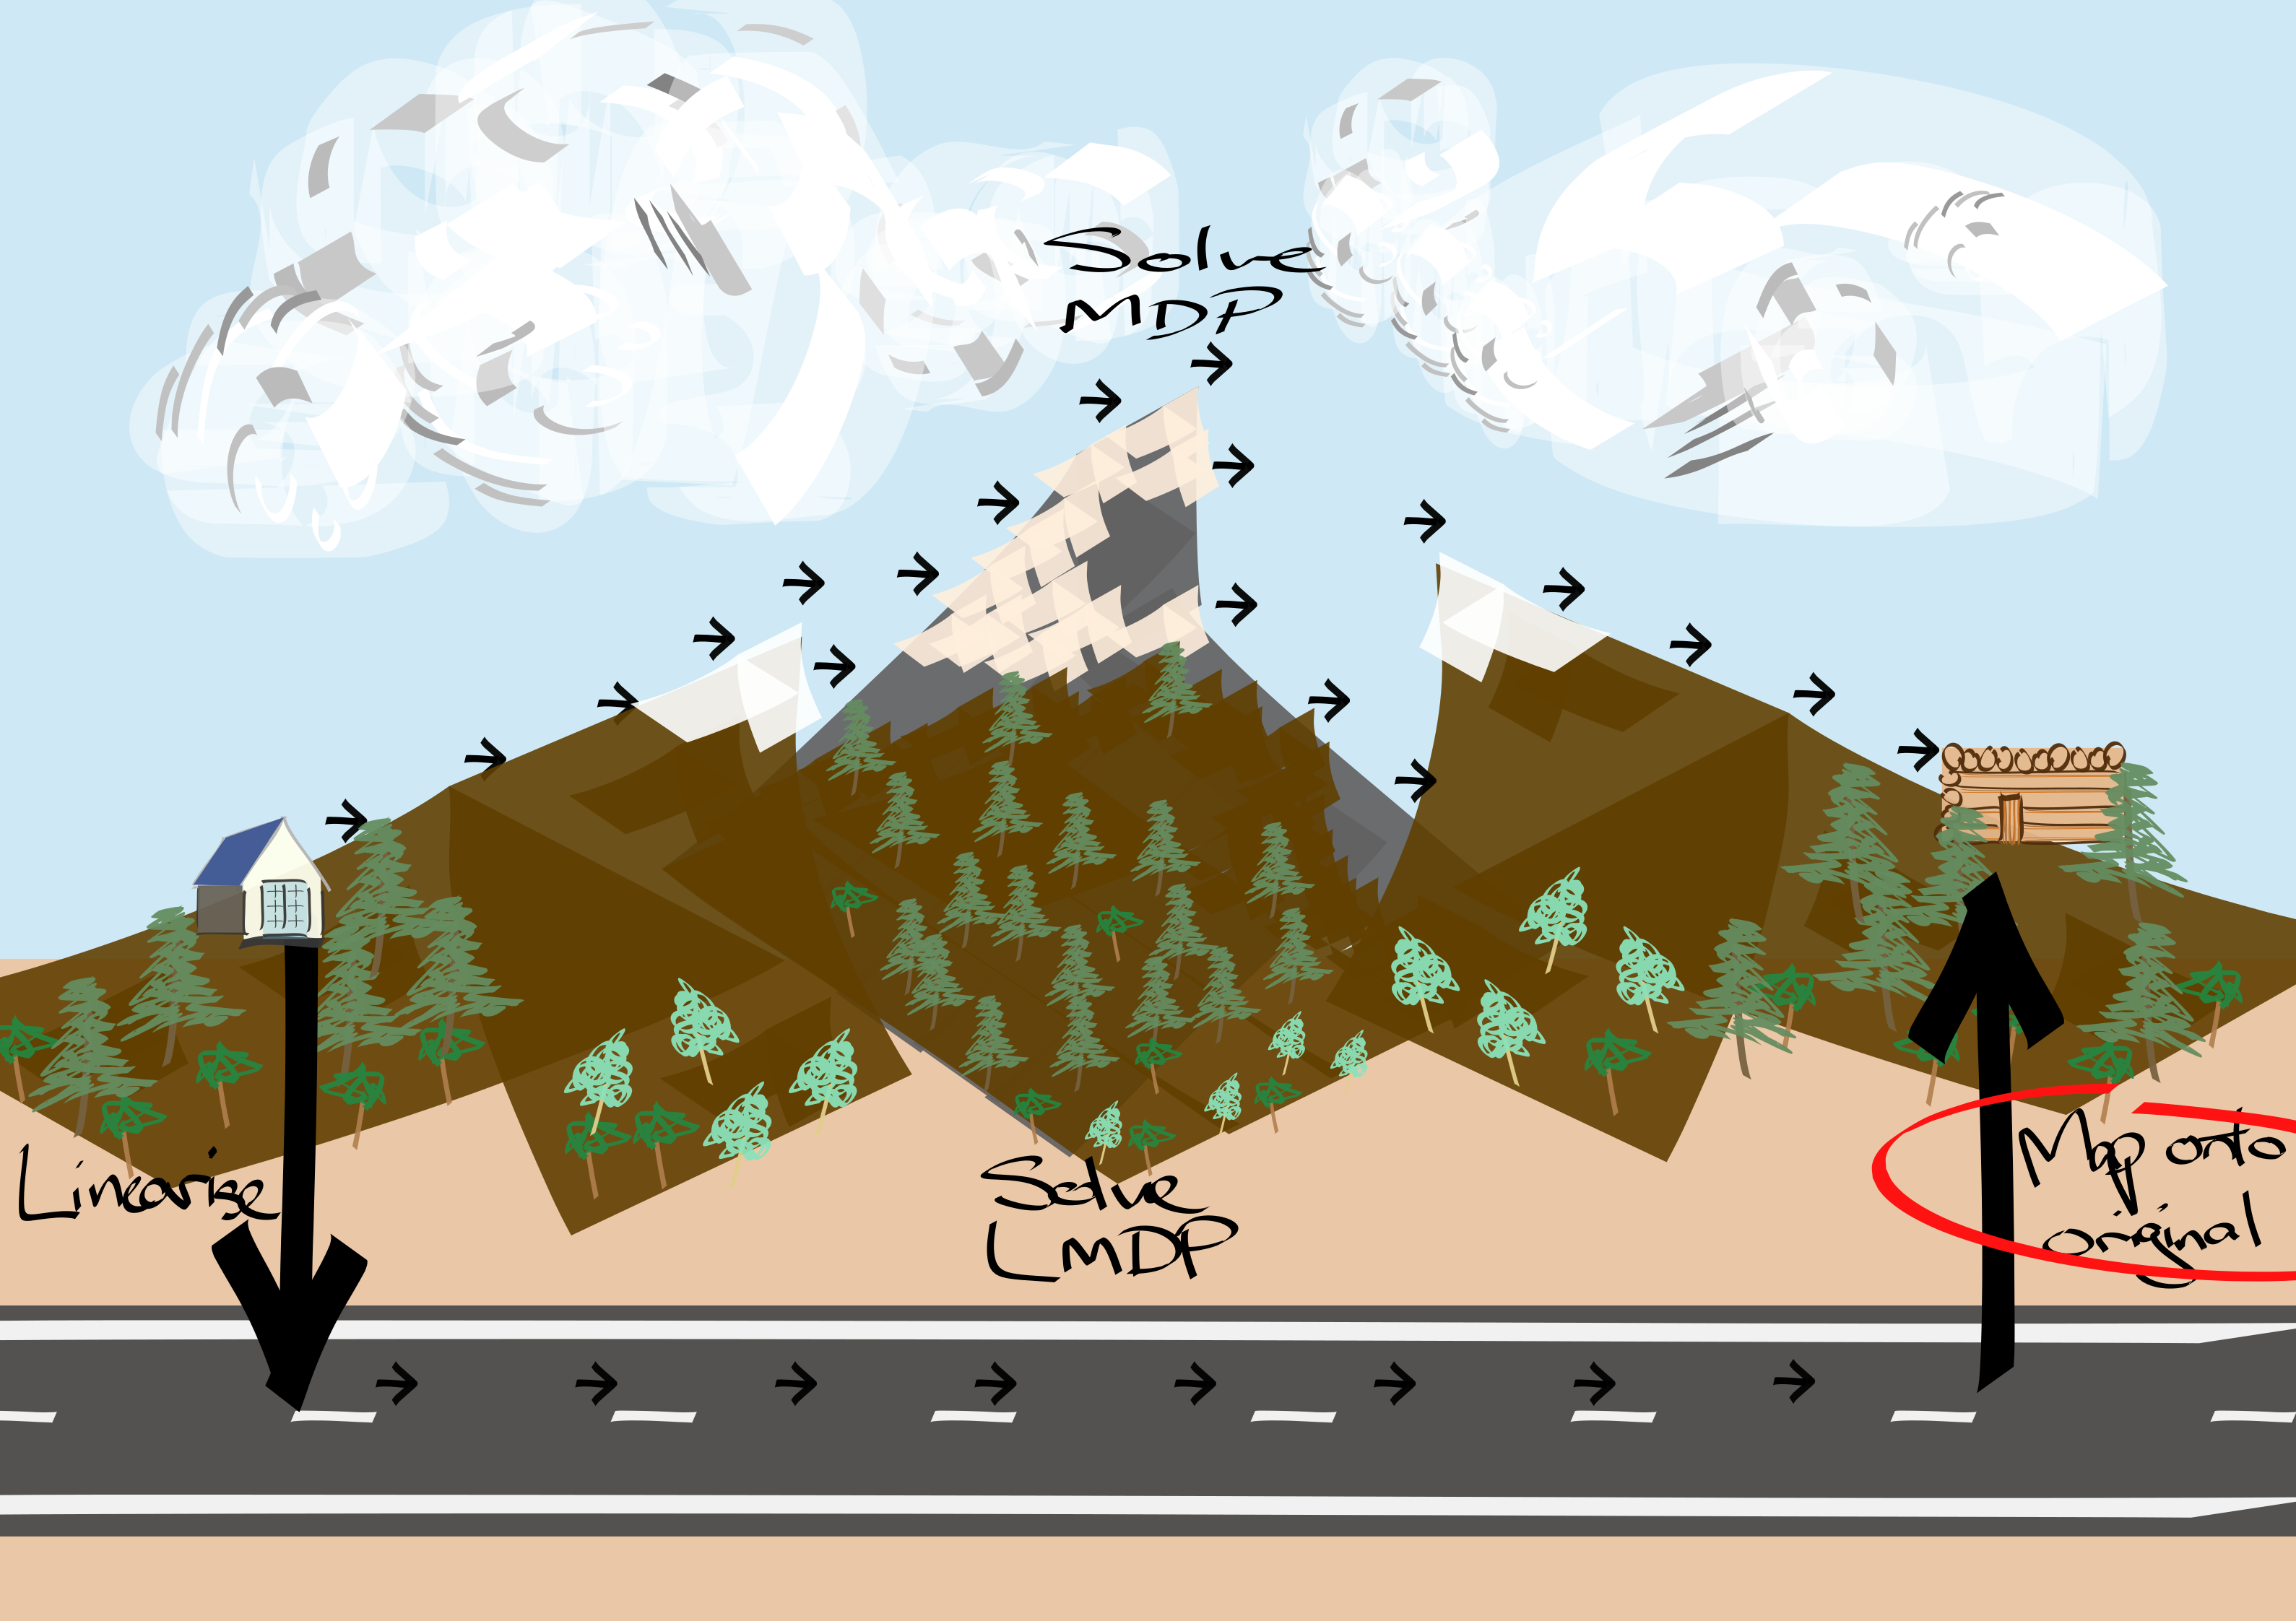
\includegraphics[width=1\textwidth,height=0.5\textheight]{../../pictures/drawings/abstract-representations-project.png}
\caption{''}
\end{figure}

Ok, so now we get a glimpse at why LMDPs are an interesting abstraction.
THe LMDP has disentangled the search for the behaviour (go to this or
that state) and the search for optimal controls (how to actually achieve
that behaviour). This can be seen in the decoding step. As we know which
states we want to be in, via the optimal control from solving the LMDP,
\(u^{* }\), but, we do not know how to implement those controls using
the actions we have available.

\begin{quote}
Two `simpler' problems. Easier to solve?
\end{quote}

\begin{align}
P_{\pi}(\cdot | s) = \sum_a P(\cdot | s, a) \pi(a | s) \\
\pi = \mathop{\text{argmin}}_{\pi} \text{KL}\Big(u(\cdot | s))\parallel P_{\pi}(\cdot | s)\Big)
\end{align}

Maybe this isnt enough? Do we need to add a reward sensitive part as
well?!? (but what if the actual path we take to get there has a neg
rewards?!?)

\hypertarget{optimality-of-solutions-via-lmdps}{%
\paragraph{Optimality of solutions via
LMDPs}\label{optimality-of-solutions-via-lmdps}}

\begin{quote}
Do these two paths lead to the same place?
\end{quote}

One of the main questions we have not addressed yet is; if we solve the
MDP directly, or linearise, solve and project, do we end up in the same
place? This is a question about the completeness of our abstraction. Can
our abstraction represent (and find) the same solutions that the
original can?

\begin{align}
\parallel V_{\pi^{* }} - \parallel V_{\pi^{* }} - V_{\pi_{u^{* }}} \parallel_{\infty}&= \epsilon  \tag{1}\\
&=\parallel (I - \gamma P_{\pi^{* }})^{-1}r_{\pi^{* }} - (I - \gamma P_{\pi_{u^{* }}})^{-1}r_{\pi_{u^{* } }} \parallel_{\infty} \tag{2}\\
&\le\parallel (I - \gamma P_{\pi^{* }})^{-1}r - (I - \gamma P_{\pi_{u^{* }}})^{-1}r \parallel_{\infty} \tag{3}\\
&=\parallel \bigg((I - \gamma P_{\pi^{* }})^{-1} - (I - \gamma P_{\pi_{u^{* }}})^{-1} \bigg) r \parallel_{\infty} \tag{4}\\
&\le r_{\text{max}} \parallel (I - \gamma P_{\pi^{* }})^{-1} - (I - \gamma P_{\pi_{u^{* }}})^{-1}   \parallel_{\infty} \tag{5}\\
&= r_{\text{max}} \parallel \sum_{t=0}^{\infty} \gamma^t P_{\pi^{* }} - \sum_{t=0}^{\infty} \gamma^t P_{\pi_{u^{* }}}  \parallel_{\infty} \tag{6}\\
&= r_{\text{max}} \parallel \sum_{t=0}^{\infty} \gamma^t (P_{\pi^{* }} - P_{\pi_{u^{* }}})   \parallel_{\infty} \tag{7}\\
&= \frac{r_{\text{max}}}{1-\gamma} \parallel P_{\pi^{* }} - P_{\pi_{u^{* }}} \parallel_{\infty} \tag{7}\\
\end{align}

\begin{enumerate}
\def\labelenumi{(\arabic{enumi})}
\tightlist
\item
  We want to compare the optimal policies value and the value achieved
  by the optimal LDMP solution.
\item
  Assume that there exists a policy that can generate the optimal
  control dynamics (as given by the LMDP). In that case we can set
  \(P_{\pi_{u^{* }}} = U^{* }\).
\item
  \(r_{u^{* }}\) doesnt really make sense as the reward is action
  dependent. We could calculate it as \(r_{\pi_{u^{* } }}\), but we dont
  explicity know \(\pi_{u^{* }}\). \((I - \gamma P_{\pi^{* }})^{-1}r\)
  represents the action-values, or \(Q\) values. By doing this exhange,
  we might over estimate the diffference under the infinity norm as two
  non-optimal actions may have larger difference. Also, use the element
  wise infinity norm.
\end{enumerate}

\begin{center}\rule{0.5\linewidth}{\linethickness}\end{center}

Ok, great. Insights from optimality bounds.

Need to be able to approximate the optimal controls. When is it hard to
approximate the optimal controls? When our basis set of distributions
oer future states (aka our actions) have little weight\ldots{}?

Potential solution? Use options.

\begin{figure}
\centering
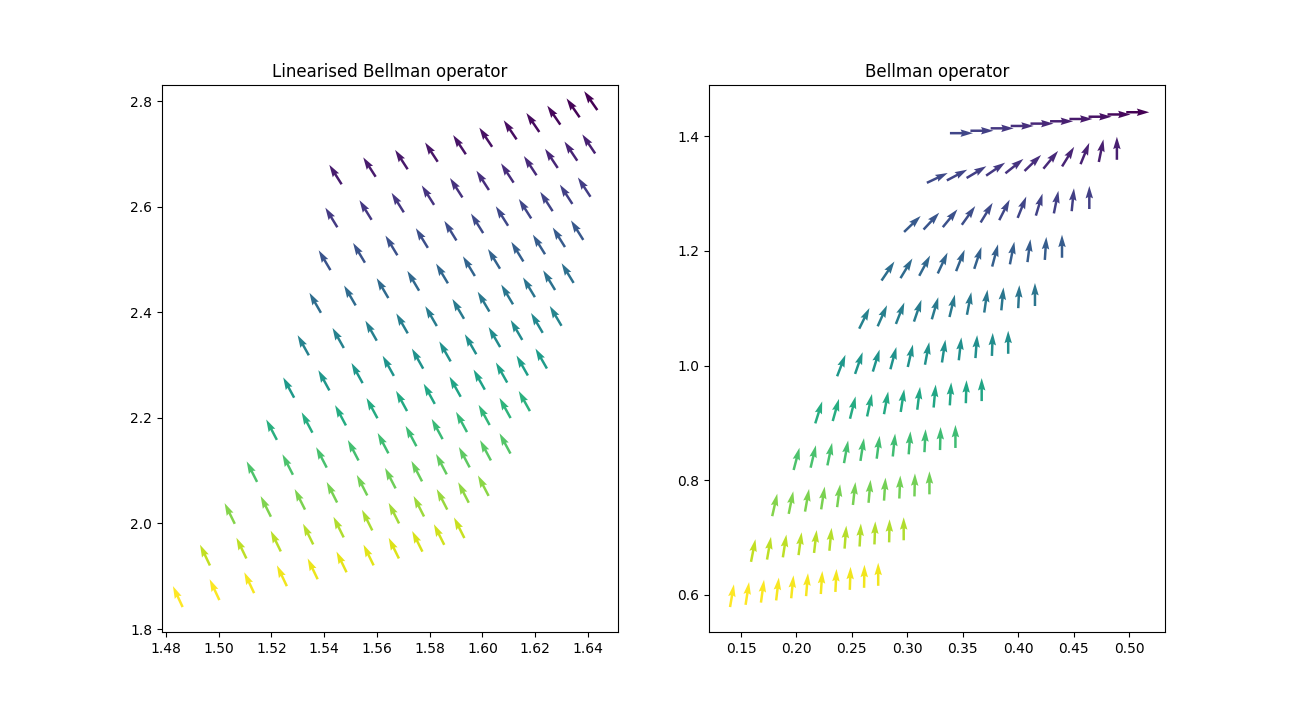
\includegraphics[width=0.75\textwidth,height=0.5\textheight]{../../pictures/figures/LBO_BO.png}
\caption{'For the same MDP, shown is a comparison of the linear temporal difference operator (left), versus the true, Bellman, temporal difference operator (right). As expected, the Bellman temporal difference operator points towards the optimal value. But, ther linear temporal difference operator points elsewhere...'}
\end{figure}

\hypertarget{option-decoding}{%
\paragraph{Option decoding}\label{option-decoding}}

What about using options to help solve the optimal control decoding?
Does this actually help?!

\begin{align}
P_{\pi}(\cdot | s) = \sum_\omega P_k(\cdot | s, \omega) \pi(\omega | s) \\
\pi = \mathop{\text{argmin}}_{\pi} \text{KL}\Big(u(\cdot | s))\parallel P_{\pi}(\cdot | s)\Big)
\end{align}

Options would allow greater flexibility in the \(P_{\pi}(\cdot | s)\)
distribution, making is possible to match \(u(s'|s)\) with greater
accuracy (and possibly cost).

\begin{itemize}
\tightlist
\item
  First need to demonstrate that action decoding is lossy.
\item
  Then show that using options is less lossy.
\end{itemize}

This introduces dangers?!? As an option might accumulate unknown rewards
along the way!??

\hypertarget{the-complexity-of-solutions-via-lmdps}{%
\subsubsection{The complexity of solutions via
LMDPs}\label{the-complexity-of-solutions-via-lmdps}}

\begin{quote}
Is my path actually shorter?
\end{quote}

The whole point of this abstraction was to make the problem easier to
solve. So hasit actually made it any easier?

The complexity of solving our abstraction can be broken down into the
three steps;

\begin{itemize}
\tightlist
\item
  linearisation: \(|S| \times \text{min}(|S|,|A|)^{2.3}\)
\item
  solve the LMDP: \(\text{min}(|S|,|A|)^{2.3}\)
\item
  project back: \(???\)
\end{itemize}

Giving a total complexity of \ldots{}

Contrasted with the complexity of solving an MDP.

\hypertarget{scaling-to-more-complex-problems}{%
\subsubsection{Scaling to more complex
problems}\label{scaling-to-more-complex-problems}}

Now that we have some evidence that this LMDP solution strategy makes
sense, it efficiently (see \href{}{complexity}) yields high value (see
\href{}{optimality}) policies. We want to test it out on some real world
problems. But the real world isn't as nice as the setting we have been
working in. There are a few added complexities;

\begin{itemize}
\tightlist
\item
  sample based / incremental
\item
  large / cts state spaces
\item
  sparse rewards
\end{itemize}

So now that we have explored LMDPs, how can we extract their nice
properties into an architecture that might scale to more complex
problems: larger state spaces and action spaces, sparse rewards,
\ldots{}?

\hypertarget{incremental-implementation}{%
\paragraph{Incremental
implementation}\label{incremental-implementation}}

Generalise to a more complex problem. We are only given samples. A first
step to tackling more complex problems.

\hypertarget{model-based}{%
\subparagraph{Model based}\label{model-based}}

Learn \(p, q\) based on samples.

\begin{align}
\mathcal L(\theta, \phi) = \mathop{\mathbb E}_{s, a,} \bigg[ r(s, a) - q_\theta(s) + \text{KL}(p_\phi(\cdot | s) \parallel P(\cdot | s, a)) \bigg]\\
\mathcal L(\theta, \phi) = \mathop{\mathbb E}_{s, r, s'} \bigg[r - q_\theta(s) - p_\phi(s' | s) \log \frac{1}{ p_\phi(s' | s)} \bigg] \\
\end{align}

\begin{center}\rule{0.5\linewidth}{\linethickness}\end{center}

Ok. Lets take a different approach. \textbf{Q:} Why is it a bad idea to
try to do incremental RL with this linearisation trick? Not sure.

\begin{center}\rule{0.5\linewidth}{\linethickness}\end{center}

Alternative perspective. The high value trajectories are the most likely
ones.

\hypertarget{distributions-over-states}{%
\subsubsection{Distributions over states}\label{distributions-over-states}}

What if we wanted to approximate these distributions? Generalise subgoal
methods to work with distributions? The distribution could be
constructed via; parzen window / GMM, neural flow, ?!.

Connections to distributional RL?

Questions

\begin{itemize}
\tightlist
\item
  What is p(s'\textbar{}s)!?!?
\item
  Want some examples of MDPs they cannot solve.
\item
  What is the relationship to other action embedding strategies?
\item
  How does p(s'\textbar{}s) bias the controls found??? I can imagine the
  unconstrained dynamics acting as a prior and prefering some controls
  over others.
\item
  If we have m states and n actions. Where m
  \textgreater{}\textgreater{} n. Then \(u(s'|s)\) is much larger than
  \(\pi(a|s)\). Also, \(u(s'|s)\) should be low rank?!
  \(u_{s's} = \sum_a u_a \alpha_a u_a^T\)
\end{itemize}

\hypertarget{other-properties}{%
\subsection{Other properties}\label{other-properties}}

LMDPs have the property that if we have already solved two LMDPs, with
the same state space, action space, unconditioned transition dynamics,
but different state rewards, \(q_1, q_2\). Then we can solve a new LMDP,
again with the same, \ldots{}, and state rewards in the span of
\(q_1, q_2\), \(z_3 = w_1 z_1 + w_2 z_2\), \ldots{}

Problem. What does it even mean for two LMDPs to have the same
unconditioned dynamics but different state rewards? The MDPs must have
been the same up to some additive constant (constant in the actions),
\(r(s, a)=r(s, a) + c(s)\). Does this really capture what we mean by
different tasks?!?

AND HRL!?!?

Refs \cite{Todorov2006,Todorov2009,Zhong,Zhonga,Dvijotham,Wozabal}



\begin{figure}
\centering
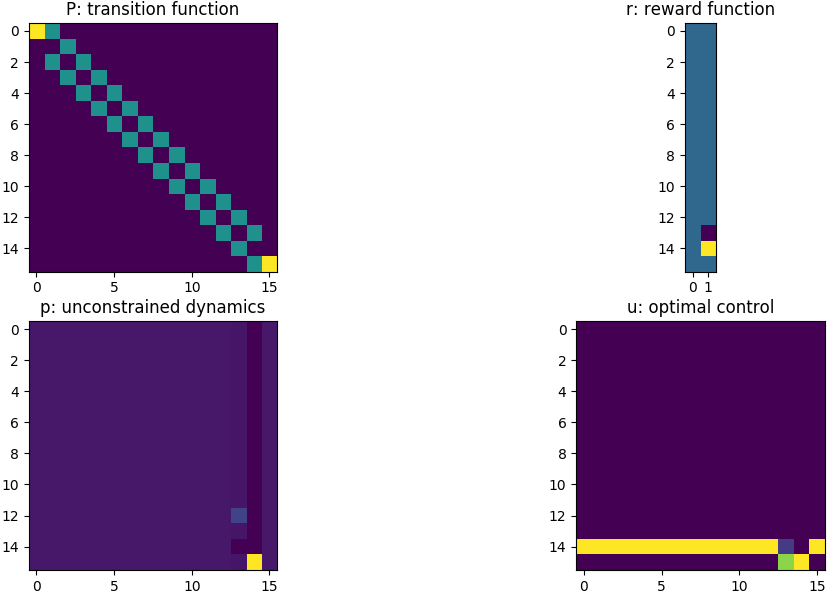
\includegraphics[width=1\textwidth,height=0.35\textheight]{../../pictures/figures/chain-test-zero-rewards.png}
\caption{A chain problem with zero reward on all states except the last two.
The optimal control to this problem is not sensible: in every state, jump to the state with positive reward.
However, it is not possible to make those transitions as }
\end{figure}

\begin{figure}
\centering
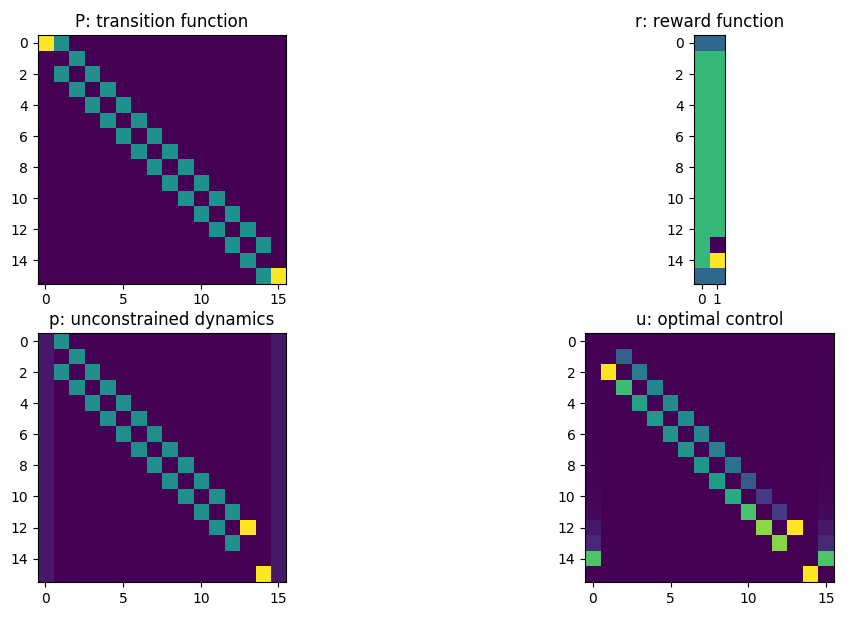
\includegraphics[width=1\textwidth,height=0.35\textheight]{../../pictures/figures/chain-test-pos-rewards.png}
\caption{A chain problem with positive rewards applied to all states.}
\end{figure}

\begin{figure}
\centering
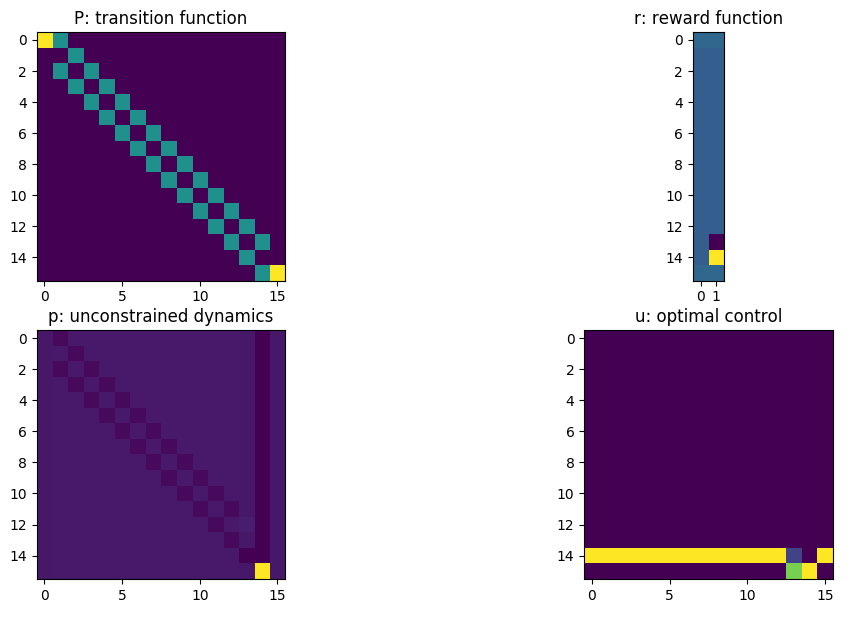
\includegraphics[width=1\textwidth,height=0.35\textheight]{../../pictures/figures/chain-test-neg-rewards.png}
\caption{A chain problem with negative rewards applied to all states}
\end{figure}

The point is, it is not entierly clear how to embed an MDP into a LMDP.
